\chapter{Parameterstudie zum Einfluss der Induktivitäten und Reglerparameter}
\label{chap:Auswertung}
Dieses Kapitel beschreibt \emph{eine} beispielhafte Anwendung des Frequenzumformermodells. Es soll mittels eines Parameterstudie untersucht werden, wie groß der Einfluss der Veränderung der Parameter der elektrischen Maschinen im Vergleich zu einer Veränderung der Reglerparameter auf das dynamische Verhalten der Anlage ist. Neben weiteren Möglichkeiten zur Auswertung des Modells (beispielsweise Systemidentifikation der Regelstrecke oder Optimierung der Maschinen- und Reglerparameter) ist aufgrund des objektorientierten und akausalen Modellierungsprinizps auch eine Einbettung des Modells in übergeordnete Modelle (z.B. zur Simulation von Verbänden mehrerer Anlagen) oder auch eine Umkehr der Kausalität (z.B. Untersuchung der Rückspeisefähigkeit, Umkehrung der Regelstrecke zum Reglerentwurf) denkbar.

\section{Problemstellung}
\label{sec:ProblemstellungParameterSweep}
Das hier untersuchte Problem entspringt der Fragestellung, ob sich das dynamische Verhalten der Anlage bei einem Lastsprung eher durch Optimieren des Reglers verbessern lässt oder eine Verbesserung nur durch Änderung der elektrischen Parameter möglich ist. Dieser zweite Fall wird zutreffen, falls der Regler bereits optimal eingestellt ist. 

Gleichzeitig bietet die Parameterstudie auch die Möglichkeit, zu untersuchen, wie die Qualität der Modellparametrierung weiter verbessert werden kann. Einige Widerstände der elektrischen Maschinen wurden bereits in \cref{chap:VerfikationValidierung} mit Hilfe der Messungen angepasst. Untersuchungen zum Abgleich der Induktivitäten der Maschinen konnten jedoch nicht durchgeführt werden. Die Parameterstudie bietet daher die Möglichkeit, zu untersuchen, welche Größen der Maschinen großen Einfluss auf das dynamische Verhalten haben und in welchen Wertebereichen eine Annäherung an die Messergebnisse erzielt werden kann.

Bewertet wird das dynamische Verhalten mit dem Integral über das Fehlerquadrat (\emph{\textbf{I}ntegrated \textbf{S}quared \textbf{E}rror} -- ISE), wobei der Fehler die Differenz zwischen der Ausgangsspannung und dem Sollwert bei einem Lastsprung ist, siehe \cref{eq:ISE}. Der ISE berücksichtigt durch das Quadrat große Abweichungen durch Schwingen stärker als andere Integralkriterien und wird in der Literatur auch als Standard zur Reglereinstellung angegeben (\cite[S.~190]{unbehauenRegelungstechnikKlassischeVerfahren2008}).
\begin{equation}
    \label{eq:ISE}
    \mathrm{ISE} = \int_0^T (115-y(t))^2 \mathrm{d}t
\end{equation}

\section{Durchführung}
In der Parameterstudie werden die Werte der elf Induktivitäten der elektrischen Maschinen einzeln variiert und ihre Auswirkung auf den ISE untersucht, wobei beachtet werden muss, dass bei der Auswahl der Parameter die reale Umsetzbarkeit \emph{nicht} berücksichtigt wurde. Für jeden Parameter werden 120 Variationen simuliert, jeweils 60 Punkte für eine Vergrößerung und 60 Punkte für eine Verkleinerung des Nennwertes. Die Verteilung der Änderung des Nennwerts wird durch eine Exponentialfunktion so beschrieben, dass der 30. Schritt den Nennwert um den Faktor 2 (also auf 50\% bzw. 200\%) ändert. Die exponentielle Verteilung wird gewählt, da sie über die festgelegte Zahl der Schritte eine Änderung der Parameter in weitem Bereich ermöglicht: Im Bereich bis zum 30. Schritt werden die Parameter nur moderat variiert, ähnlich einer linearen Verteilung, ab dem 30. Schritt jedoch ist die Änderung durch die exponentielle Verteilung größer als die der linearen Verteilung. Die Werte nähern sich einer quadratischen Verteilung an (siehe \cref{fig:VerteilungParameter}).
\begin{figure}
    \centering
    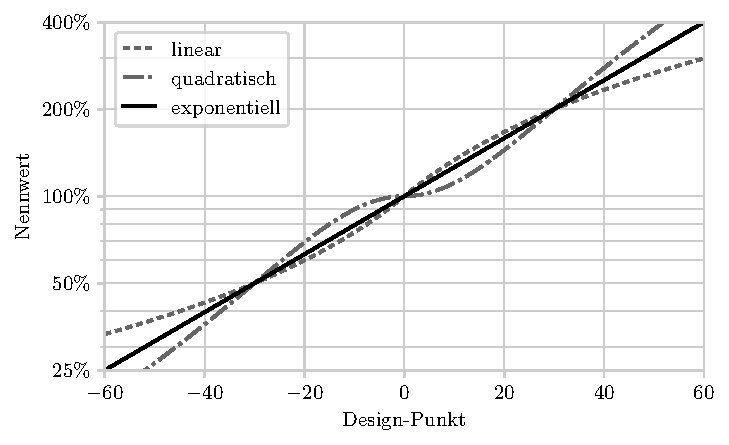
\includegraphics[width=.8\textwidth]{Bilder/verteilung_log.pdf}
    \caption{Verschiedene Verteilungsfunktionen zur Parametervariation}
    \label{fig:VerteilungParameter}
\end{figure}

Durchgeführt wird die Parameterstudie mit Hilfe eines Python-Skripts (siehe \cref{lst:ModelicaSweep}). Das kompilierte Modell des Frequenzumformers wird mit dem Skript gestartet und der geänderte Parameter zugewiesen. Das Modell wird für \unit[3]{s} simuliert. Bei $t=\unit[2,2]{s}$ wird ein Lastsprung von \unit[50]{\%} auf \unit[100]{\%} ausgeführt. Anschließend werden die Simulationsergebnisse in Python eingelesen und der ISE (vgl. \cref{eq:ISE}) vom Sprungbeginn an  über ein Intervall von $T=\unit[0,8]{s}$ berechnet, bis die Ausgangsspannung (bei Nennparametern) den stationären Zustand erreicht. Zusätzlich zu der Parameterstudie über die Induktivitäten der elektrischen Maschinen wurde auch eine Parameterstudie mit veränderten Reglerparametern wie in der dynamischen Messung in \cref{sec:Messaufbau} durchgeführt.

\section{Ergebnisse}
Die aus der Parameterstudie der Induktivitäten resultierenden Zeitverläufe der Spannungen zeigen \cref{fig:InduktivitatenSweepA,fig:InduktivitatenSweepB}. Die Spannungsverläufe aus der Studie der Reglerparameter zeigt \cref{fig:SpannungenReglerSweep}.

Die Zeitverläufe der Spannungen geben einen Überblick über den Einfluss der einzelnen Induktivitäten auf das dynamische Verhalten. So ist zu erkennen, dass die Induktivitäten der Asynchronmaschine generell kaum Einfluss nehmen auf die Spannungsverläufe. Ebenso ist auch der Einfluss der Induktivitäten bezüglich der q-Achse generell geringer als derjenige der entsprechenden Induktivität bezüglich der d-Achse. Den größten Einfluss auf den Spannungsverlauf haben demnach die Hauptinduktivitäten $L_{\mathrm{md}}$ der beiden Synchronmaschinen, die bei großen Minderungen der Induktivitäten einen stationären Regelfehler aufweisen.

Die Einflüsse der weiteren Induktivitäten der beiden Synchronmaschinen sind wesentlich geringer und verteilen sich auf unterschiedliche Weise, wobei auch beachtet werden muss, dass die Rotorstreuinduktivitäten $L_{\mathrm{r\sigma}}$ bei der Erregermaschine nicht auftreten, da diese ohne Dämpferkäfig ausgeführt ist. Nach der Hauptinduktivität bezüglich der d-Achse haben bei dem Synchrongenerator die Streuinduktivität des Stators und die Streuinduktivität des Rotors bezüglich der d-Achse den größten Einfluss auf das dynamische Verhalten, bei der Erregermaschine hingegen ist der Einfluss der Hauptinduktivität bezüglich der q-Achse etwas größer als der Einfluss der Streuinduktivität, wobei der Unterschied sich vor Allem in der Dämpfung und der Frequenz des Schwingungsanteils zeigt. 

Ein Vergleich mit den gemessenen Spannungsverläufen in \cref{fig:ZeitverlauefeSpannungenParametersweep} zeigt eine Annäherung der Simulation an die Messung bei moderater Verringerung der Hauptinduktivitäten bezüglich der d-Achse der beiden Synchronmaschinen.

\begin{figure}
    \captionsetup[subfigure]{aboveskip=1pt,belowskip=1pt}
    \centering
    \begin{subfigure}{\textwidth}
        \centering
        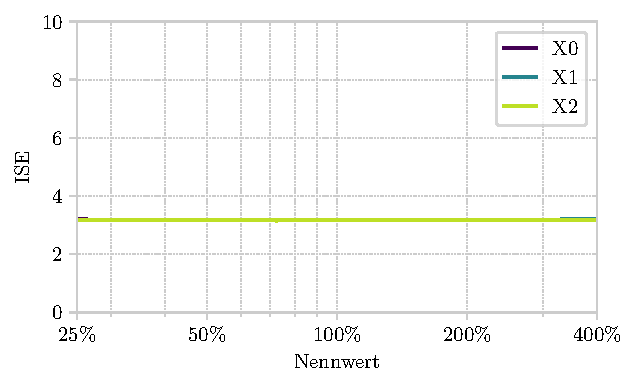
\includegraphics{Bilder/aimc_ISE.pdf}
        \caption{ASM}
        \label{fig:ISE_ASM}
    \end{subfigure}
    \begin{subfigure}{\textwidth}
        \centering
        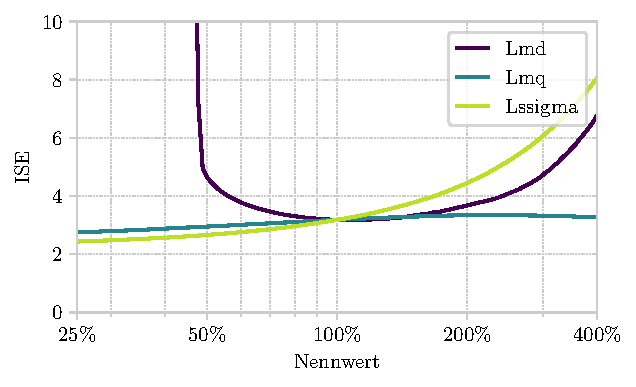
\includegraphics{Bilder/smee_ISE.pdf}
        \caption{Synchrongenerator}
        \label{fig:ISE_SG}    
    \end{subfigure}
%     \caption{Einfluss der Induktivitäten auf den ISE}
% \end{figure}
% \begin{figure}\ContinuedFloat
%     \centering
    \begin{subfigure}{\textwidth}
        \centering
        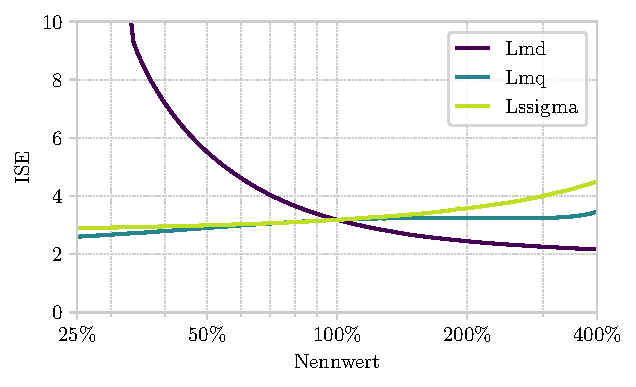
\includegraphics{Bilder/sM_E_ISE.pdf}
        \caption{Erregermaschine }
        \label{fig:ISE_ERR}    
    \end{subfigure}
    \caption{Einfluss der Induktivitäten auf den ISE}
\end{figure}
\begin{figure}
    \centering
    \begin{subfigure}{.49\linewidth}
        \centering
        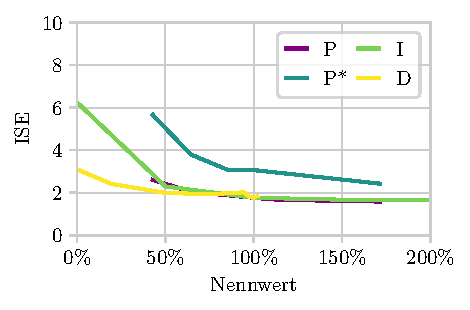
\includegraphics{Bilder/regler_ISE.pdf}    
        \subcaption{Messung}
    \end{subfigure}
    \begin{subfigure}{.49\linewidth}
        \centering
        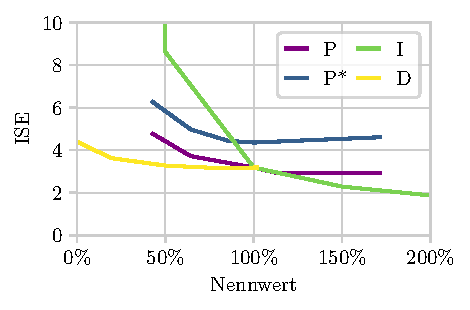
\includegraphics{Bilder/simulation_reglerSweep.pdf}
        \subcaption{Simulation}
    \end{subfigure}
    \caption{Einfluss der Reglerparameter auf den ISE}
    \label{fig:ISE_ReglerSweep}
\end{figure}

Der Einfluss der Induktivitäten und der Reglerparameter auf das dynamische Verhalten kann auch aus dem resultierenden ISE abgelesen werden. Die \cref{fig:ISE_ASM,fig:ISE_ERR,fig:ISE_SG} zeigen den Verlauf des ISE bei Veränderung der Induktivitäten. Der große Einfluss der Hauptinduktivitäten $L_{\mathrm{md}}$ der Synchronmaschinen zeigt sich im Verlauf des ISE. Der Knick im Verlauf des ISE bei ca \unit[50]{\%} bzw. \unit[33]{\%} des Nennwerts lässt sich begründen mit der beobachteten stationären Abweichung der Spannungen. Alle Verringerungen des ISE hingegen sind von kleinem Ausmaß.

Bei der Bewertung dieser stationären Abweichungen muss berücksichtigt werden, dass diese durch den Begrenzer des Spannungsreglers hervorgerufen wird, der einer Parametrierungsunsicherheit unterliegt. Die Reglerparameter sind gesichert, jedoch unterliegt die Umwandlung der reglerinternen Stellgröße auf die Ausgangsspannung einer unsicheren Datenlage. So kann die maximal mögliche Stellspannung um den Faktor 1,25 bis 1,5 nach oben abweichen, in Abhängigkeit von der gewählten maximalen Stellspannung (siehe \cref{sec:AbbildungReglerZahlen}. Mit einer größeren maximal möglichen Stellspannung würde auch der stationäre Regelfehler kleiner werden. Solange der Spannungsregler jedoch nicht bis zum Begrenzer aussteuert, beeinflusst dieser Fehler das dynamische Verhalten kaum.

Zum Vergleich der aus der dynamischen Messung mit Reglerveränderung erhaltenen Ergebnisse mit dem Simulationsmodell, wurden die entsprechenden Messparameter ebenfalls in der Simulation untersucht, mit derselben Methode wie bei den Induktivitäten (siehe \cref{fig:ISE_ReglerSweep,}). Der absolute Unterschied des ISE zwischen Simulation und Messung erklärt sich aus dem verbliebenen Modellierungs- und Parametrierungsfehler des Simulationsmodells. Es zeigt sich aber, dass das Trendverhalten der Reglerparameter in Simulation und Messung ähnlich sind. Die geringen Verminderungen des ISE (vor Allem in der Messung) zeigen, dass der Regler bereits gut, das heißt nahe eines lokalen Minimums des ISE eingestellt ist. Zum Nachweis des globalen Minimums wären weitere Untersuchungen hinsichtlich der Konvexität des Minimierungsproblems notwendig (siehe dazu \cite{eschVerfahrenZurGuteoptimalen2016}).

Den größten Einfluss auf den ISE nimmt die Verstärkung des I-Anteils. Generell bewirkt der I-Anteil des PID-Reglers stationäre Genauigkeit. Wird die Verstärkung des I-Anteils verringert, kann der Regler nicht mehr oder nicht in demselben Zeitraum den Regelfehler ausgleichen. Ähnlich wie bei den Hauptinduktivitäten der Synchronmaschinen zeigt sich diese bleibende Abweichung in dem hohen ISE. Der hohe Einfluss des P-Anteils ($P^*$) erklärt sich aus dem höheren Fehler im unveränderten Zustand durch den fehlenden D-Anteil (Konfiguration als PI-Regler). Wird dieser Startfehler berücksichtigt (vertikales Verschieben der Kurve), zeigt sich ein ähnliches Verhalten, wie bei Konfiguration als PID-Regler. Der Einfluss des P-Anteils und des D-Anteils fällt im Vergleich zum I-Anteil geringer aus, wobei der P-Anteil größeren Einfluss nimmt als der D-Anteil.

Zum Vergleich des Einflusses der Reglerparameter mit dem Einfluss der Induktivitäten auf den ISE wird die prozentuale Änderung des ISE bei Änderung eines Parameters um den Faktor 2 untersucht, das heißt in den Bereichen $[\unit[50]{\%},\unit[100]{\%}]$ und $[\unit[100]{\%},\unit[200]{\%}]$ des Nennwerts. Da die Reglerparameter nicht alle bis \unit[200]{\%} variiert wurden, werden die Verläufe des $P$-, $P^*$- und $I$-Anteils linear extrapoliert. Der ISE des $D$-Anteils hingegen wird nur im Intervall $[\unit[50]{\%},\unit[100]{\%}]$ ausgewertet, da im $[\unit[100]{\%},\unit[200]{\%}]$ Intervall zu wenig Parameter untersucht wurden. Für jeden Parameter mit Ausnahme des $D$-Anteils ergeben sich also zwei prozentuale Änderungen. Berechnet wird die prozentuale Änderung des ISE mit Hilfe des Skripts in \cref{lst:Trendanalyse,lst:TrendanalyseCommand}. Die Ergebnisse aus Simulation und Messung für die Induktivitäten und die Reglerparameter sind in \cref{fig:trend_manager_scatter} dargestellt.
\begin{figure}
    \centering
    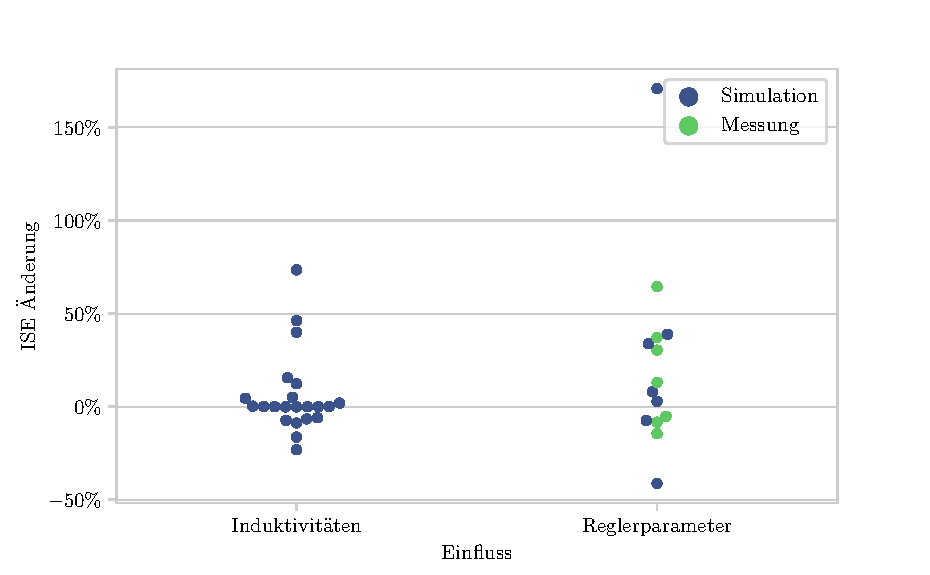
\includegraphics{Bilder/trend_manager_scatter.pdf}
    \caption{Prozentuale Änderung des ISE bei Variation jedes Parameters um Faktor 2}
    \label{fig:trend_manager_scatter}
\end{figure}

Es zeigt sich, dass in dem untersuchten Parameterbereich die Induktivitäten und die Reglerparameter einen ähnlich großen Einfluss auf den ISE nehmen. Minimierung des ISE (d.h. Verbesserung des dynamischen Verhaltens) ist sowohl durch Variation der Induktivitäten als auch der Reglerparameter möglich. Das Potential zur Minimierung des ISE ist kleiner als das zur Vergrößerung. Das bedeutet, dass die aktuelle Parametrierung des Frequenzumformers sich nahe eines (zumindest lokalen) Minimums befindet. Die Parameter der Simulation weisen größeres Potential zur Verbesserung auf als die Messung, was durch den Modellierungsfehler erklärt wird. 

Diese Erkenntnisse können in der Auslegung und Regelung angewendet werden. Zunächst kann festgestellt werden, dass sowohl der Einfluss der Maschinenparameter als auch der der Reglerparameter im Entwurf berücksichtigt werden sollte, da beide ähnlich großen Einfluss auf das dynamische Verhalten nehmen. Dann ist aber auch offensichtlich, dass die beliebige Änderung der Reglerparameter mit vernachlässigbaren Kosten einhergeht, während eine Änderung der Induktivitäten nicht in beliebigem Rahmen möglich ist und mit hohen Entwicklungs- und Materialkosten verbunden ist. Daher empfiehlt es sich, zur Optimierung zuerst das Potential der Reglerparameter auszuschöpfen. Schlussendlich ergibt sich die Möglichkeit, Materialeinsparungen an den elektrischen Maschinen durch Erhöhung des ISE zu erkaufen und die Erhöhung durch Optimierung der Reglerparameter auszugleichen und trotzdem ein gutes (d.h. die Anforderungen erfüllendes) dynamisches Verhalten zu erzielen.

%% Trendanalyse mit Steigung:
% Zum Vergleich des Einflusses der Reglerparameter mit dem Einfluss der Induktivitäten auf den ISE wird die durchschnittliche Steigung des ISE in den Bereichen $[\unit[50]{\%},\unit[100]{\%}]$ und $[\unit[100]{\%},\unit[200]{\%}]$ des Nennwerts untersucht. Die durchschnittliche Steigung über einem Intervall ergibt sich nach \cref{eq:mittlereSteigung} aus dem Differenzenquotient der Intervallgrenzen. 
% \begin{equation}
%     \label{eq:mittlereSteigung}
%     \Bar{m} = \frac{1}{T} \int_{t_0}^{t_0+T} f'(t) \mathrm{d}t = \frac{f(t_0+T) - f(t_0)}{T}
% \end{equation}
% Berechnet wird die durchschnittliche Steigung für den ISE der Parameter mit Hilfe des Skripts in \cref{lst:Trendanalyse,lst:TrendanalyseCommand}. Die Ergebnisse aus Simulation und Messung für die Induktivitäten und die Reglerparameter zeigt \cref{fig:trend_manager_scatter}.